\Exercise{Video und Canvas – Gemeinsam mehr erreichen}
%
\par Canvas an sich wäre schon fast langweilig wenn da nicht noch das neue
Videoelement hinzukäme. In dieser Aufgabe verbinden Sie die beiden Elemente um
einen sehr einfachen dynamischen Effekt zu erzeugen. Was Sie dazu brauchen ist
eine Webseite mit einem \htag{canvas}-Element, einem nicht angezeigten
\htag{div}, welches ein \htag{video} sowie ein weiteres \htag{canvas} enthält und
ein wenig JavaScript. Verwenden Sie als Videoquellen wieder das bereits
bekannte Synergy Video aus Aufgabe 18.
%
\par Folgender Aufbau ist hilfreich: \\Setzen Sie die Attribute des
\htag{video}-Elements \jvar{autoplay=true} und \jvar{loop=true}. Sobald das
Video geladen hat sollten Sie dann in entsprechenden Abständen (z.B. in
\qty{40}{ms} Pulsen) in das (versteckte, d.h. im \htag{div}-Container
enhaltene) Canvas zeichnen. Übergeben Sie hierzu einfach das Videoelement der
\jfunc{drawImage} Methode des Canvas Contexts:
%
\begin{lstlisting}
mycontext.drawImage(bild, sx, sy, sw, sh, dx, dy, dw, dh);
\end{lstlisting}
%
\par Abschließend zeichnen Sie auf das (sichtbare) Canvas. Hierzu sollen Sie
folgendermaßen vorgehen:
%
\begin{figure}
\centering
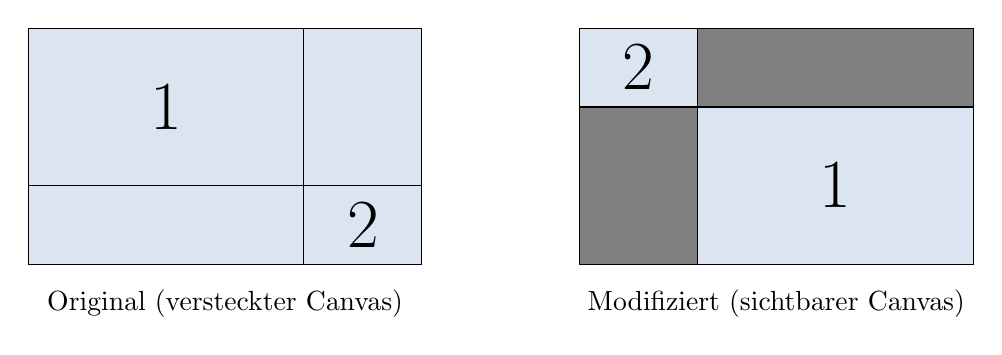
\begin{tikzpicture}

\definecolor{myblue}{RGB}{219,229,241}
\definecolor{mygray}{RGB}{128,128,128}

    %Farben
    \fill [myblue] (0,0) rectangle (5,3);

    %Rechteck mit Kreuz
    \draw (0,0) -- ++(5,0) -- ++(0,3) -- ++(-5,0) -- cycle;
    \draw (3.5,0) -- ++(0,3);
    \draw (0,1) -- ++(5,0);
    
    %Labels
    \node at (1.75,2) {\Huge 1};
    \node at (4.25,0.5) {\Huge 2};
    \node at (2.5,-.5) {Original (versteckter Canvas)};
    
%Rechte Seite
\begin{scope}[xshift=7cm]

    %Farben
    \fill [myblue] (0,0) rectangle (5,3);
    \fill [mygray] (1.5,2) rectangle (5,3);
    \fill [mygray] (0,0) rectangle (1.5,2);
    
    %Rechteck mit Kreuz
    \draw (0,0) -- ++(5,0) -- ++(0,3) -- ++(-5,0) -- cycle;
    \draw (1.5,0) -- ++(0,3);
    \draw (0,2) -- ++(5,0);
    
    %Labels
    \node at (0.75,2.5) {\Huge 2};
    \node at (3.25,1) {\Huge 1};
    \node at (2.5,-.5) {Modifiziert (sichtbarer Canvas)};
    
\end{scope}
\end{tikzpicture}
\end{figure} 

\par Dies bedeutet, dass Sie zwei Ausschnitte aus dem Videobild versetzt
zeichnen und den Rest mit einer entsprechenden Füllung versehen. Diese muss
nicht einheitlich sein, sondern kann von Ihnen frei entschieden werden.